
\documentclass{article} % For LaTeX2e
\usepackage{iclr2026_conference,times}

% Optional math commands from https://github.com/goodfeli/dlbook_notation.
\input{math_commands.tex}

% zjx packages
\usepackage{hyperref}
\usepackage{url}
\usepackage{enumitem}
\usepackage{xcolor}
\usepackage{graphicx}
\usepackage{booktabs}
\usepackage{multirow}
\usepackage[table]{xcolor}
\usepackage{subcaption}
\usepackage{tcolorbox}
\usepackage{textcomp}
\usepackage[T1]{fontenc}
\tcbuselibrary{theorems,breakable,skins}
\newtcbtheorem[]{myexample}{Example}%
{
  breakable,
  enhanced,
  colback=green!5,
  colframe=green!35!black,
  fonttitle=\bfseries,
  % Adjust internal padding
  top=2pt,         % Space between top frame and content
  bottom=2pt,      % Space between bottom frame and content
  % Adjust external margin
  before skip=4pt, % Space before the box
  after skip=4pt   % Space after the box
}{th}


\title{Reasoning-Enhanced Large Language Models for Molecular Property Prediction}

% Authors must not appear in the submitted version. They should be hidden
% as long as the \iclrfinalcopy macro remains commented out below.
% Non-anonymous submissions will be rejected without review.


\author{
    Jiaxi Zhuang$^{1*}$, Yaorui Shi$^{1*}$, Jue Hou$^{1*}$, Yunong He$^1$, Mingwei Ye$^1$, Mingjun Xu$^1$, \\
    \normalsize
    \textbf{Yuming Su$^1$, Linfeng Zhang$^2$, Linfeng Zhang$^1$, Guolin Ke$^1$, Hengxing Cai$^{1\dagger}$} \\
    $^1$DP Technology; \quad $^2$ Shanghai Jiao Tong University; \\ $^{*}$Equal contribution; \quad $^{\dagger}$Corresponding author.
    %\\ \small{\texttt{\{zhuangjiaxi, caihengxing\}@dp.tech}}
}

% \author{
%   Haitao Lin$^{1,3, \dag}$, \quad Guojiang Zhao$^{2, \dag}$, \quad Odin Zhang$^3$, \quad Yufei Huang$^1$, \\
%   \textbf{  Lirong Wu$^1$, \quad Zicheng Liu$^1$, \quad Siyuan Li$^1$,\quad  Cheng Tan$^1$, \quad Zhifeng Gao$^2$, \quad Stan Z. Li$^{1, *}$}  \\
%   $^1$ AI Lab, Research Center for Industries of the Future, Westlake University; \\
%   $^2$ DP Technology; \quad $^3$ Zhejiang University; \quad $^\dag$ Equal Contribution; \quad $^{*}$ Corresponding Author. \\
%   \texttt{linhaitao@westlake.edu.cn}
% }


% \author{Antiquus S.~Hippocampus, Natalia Cerebro \& Amelie P. Amygdale \thanks{ Use footnote for providing further information
% about author (webpage, alternative address)---\emph{not} for acknowledging
% funding agencies.  Funding acknowledgements go at the end of the paper.} \\
% Department of Computer Science\\
% Cranberry-Lemon University\\
% Pittsburgh, PA 15213, USA \\
% \texttt{\{hippo,brain,jen\}@cs.cranberry-lemon.edu} \\
% \And
% Ji Q. Ren \& Yevgeny LeNet \\
% Department of Computational Neuroscience \\
% University of the Witwatersrand \\
% Joburg, South Africa \\
% \texttt{\{robot,net\}@wits.ac.za} \\
% \AND
% Coauthor \\
% Affiliation \\
% Address \\
% \texttt{email}
% }

% The \author macro works with any number of authors. There are two commands
% used to separate the names and addresses of multiple authors: \And and \AND.
%
% Using \And between authors leaves it to \LaTeX{} to determine where to break
% the lines. Using \AND forces a linebreak at that point. So, if \LaTeX{}
% puts 3 of 4 authors names on the first line, and the last on the second
% line, try using \AND instead of \And before the third author name.

\newcommand{\fix}{\marginpar{FIX}}
\newcommand{\new}{\marginpar{NEW}}
\newcommand{\todo}[1]{\textbf{\textcolor{red}{TODO: #1}}}

\iclrfinalcopy % Uncomment for camera-ready version, but NOT for submission.
\begin{document}


\maketitle

\begin{abstract}
Molecular property prediction is crucial for drug discovery and materials science, yet existing approaches suffer from limited interpretability, poor cross-task generalization, and lack of chemical reasoning capabilities. Traditional machine learning models struggle with task transferability, while specialized molecular language models provide little insight into their decision-making processes. To address these limitations, we propose \textbf{MPPReasoner}, a multimodal large language model that incorporates chemical reasoning for molecular property prediction.
Our approach, built upon Qwen2.5-VL-7B-Instruct, integrates molecular images with SMILES strings to enable comprehensive molecular understanding. We develop a two-stage training strategy: supervised fine-tuning (SFT) using 16,000 high-quality reasoning trajectories generated through expert knowledge and multiple teacher models, followed by Reinforcement Learning from Principle-Guided Rewards (RLPGR). RLPGR employs verifiable, rule-based rewards that systematically evaluate chemical principle application, molecular structure analysis, and logical consistency through computational verification.
Extensive experiments across 8 datasets demonstrate significant performance improvements, with MPPReasoner outperforming the best baselines by 7.91\% and 4.53\% on in-distribution and out-of-distribution tasks respectively. MPPReasoner exhibits exceptional cross-task generalization and generates chemically sound reasoning paths that provide valuable insights into molecular property analysis, substantially enhancing both interpretability and practical utility for chemists.
Code is available at \url{https://anonymous.4open.science/r/MPPReasoner-12687}.
\end{abstract}

\section{Introduction}
\label{sec:intro}

\begin{figure}
    \centering
    \includegraphics[width=\linewidth]{figs/fig_immer_demo.pdf}
    \caption{Comparison between (a) classical IR that acquires on-axis data in controlled setups with dedicated sensors, and (b) immersive IR that acquires off-axis data in open scenes with VR headsets. Examples are from CASIA-IrisV4~\cite{casia-iris-v4} and ImmerIris.}
    \label{fig:immer-demo}
    \vspace{-3mm}
\end{figure}

% Iris recognition is a long-standing biometric technique that identifies persons by comparing the unique texture patterns of their irises. The iris is a thin, circular structure in the human eye that regulates the amount of light reaching the retina. Its texture, readily capturable in ocular images, is randomly formed, highly distinctive, and relatively stable over time, making iris secure and accurate for personal identification. In recent years, with the rise of egocentric applications such as augmented reality (AR) and virtual reality (VR), IR has gained renewed prominence, as irises can be seamlessly captured through home electronics like VR headsets, offering convenience in scenarios such as login and e-pay. We refer to this emerging scenario as \textit{immersive IR}, to distinguish it from classical IR in controlled setups. \Cref{fig:immer-demo} compares the acquisition scenario and example images between two setups.

Iris recognition is a long-standing biometric technique that identifies persons by the unique patterns of their irises. The iris is a thin, circular structure in the human eye that regulates the amount of light reaching the retina. Its texture, being randomly formed, highly distinctive, and relatively stable over time, provides a secure and accurate basis for personal identification. \textit{Classical} iris recognition (\cref{fig:immer-demo}(a)) has long been employed in sensitive applications such as access control. More recently, with the rise of egocentric applications such as augmented reality (AR) and virtual reality (VR), \textit{immersive} iris recognition (\cref{fig:immer-demo}(b)) has gained renewed prominence, as irises can be conveniently acquired through consumer electronics such as VR headsets to enable seamless use in tasks like login and e-payment.

Immersive and classical iris recognition differ most clearly in how data are acquired. Classical iris recognition is a controlled setup that uses specialized frontal cameras to capture on-axis images under full user cooperation. In contrast, the immersive setup places cameras at a tilt on headsets due to hardware design and user experience, producing off-axis images. Acquisition also takes place in open scenes, where environments vary and non-expert users cooperate less consistently. Together, off-axis and open-scene acquisition give rise to 3 distinctive challenges: 1) \textit{Perspective distortion}, where tilted camera-eye geometries make the circular iris appear elliptical and stretch local textures; (2) \textit{Quality degradation}, where the absence of control in device calibration and user cooperation can yield flawed samples, \eg, occlusions when eyes are not fully opened; and 3) \textit{Intra-class variation}, which arises from environmental and behavioral changes in such as illumination and gaze direction. Data scarcity has long been a barrier for iris recognition research, with most existing datasets proprietary or small in scale. For immersive iris recognition, which is still an emerging topic, datasets capturing these challenges are even scarcer.

% Immersive and classic iris recognition differ fundamentally in data acquisition. Classic iris recognition, as a controlled setup, uses frontal cameras to capture on-axis iris images under full user cooperation. By contrast, the immersive setup employs tilt-placed headset cameras to avoid obstructing the display, producing off-axis images, and acquisition often takes place in open scenes where environments vary and non-expert users cannot be expected to cooperate consistently. Off-axis and open-scene acquisition therefore introduce 3 distinctive challenges: 1) \textit{Perspective distortion}, where tilted camera-eye geometries cause circular irises to appear elliptical and local textures to be unevenly stretched; 2) \textit{Quality degradation}, as casual wearing or calibration often produce defocused images, while inconsistent cooperation can lead to partial occlusions from eyelids or eyelashes; and (3) \textit{Intra-class variation}, where environmental and behavioral factors such as illumination changes and gaze direction shifts can induce substantial variations. Data scarcity has long been a barrier for iris recognition research, with most existing datasets being proprietary or small in scale. For immersive iris recognition, this issue is even more pronounced.


% Iris recognition is a long-standing biometric technique that identifies persons by the unique texture patterns of their irises. The iris is a thin, circular structure in the human eye that regulates the amount of light reaching the retina. Its texture, being randomly formed, highly distinctive, and relatively stable over time, is secure and accurate for personal identification. \textit{Classic} iris recognition (\cref{fig:immer-demo}(a)) has long been employed in sensitive applications such as access control, where a dedicated frontal camera captures on-axis iris images under controlled setups with full user cooperation. More recently, with the rise of egocentric applications such as augmented reality (AR) and virtual reality (VR), \textit{immersive} iris recognition (\cref{fig:immer-demo}(b)) has gained renewed prominence, as irises are captured through consumer VR headsets for convenient login and e-payment. Unlike the classic setting, headset cameras are usually tilt-placed to avoid obstructing the display, producing off-axis images, and acquisition occurs in open scenes where environments vary and users, being non-experts, cannot be expected to cooperate in a controlled manner.

% Data scarcity has long been a critical barrier for iris recognition research. In classical settings, collecting data requires costly specialized devices, hence existing datasets are mostly proprietary or small in scale. For immersive iris recognition, the problem is even more pronounced due to 3 distinctive challenges of open-scene iris acquisition: 1) \textit{Off-axis distortion.} VR/AR headsets typically capture tilted or off-axis ocular images, where perspective distortion, \eg, the circular iris appearing elliptical and local textures being unevenly stretched, can undermine the geometric consistency of iris textures. 2) \textit{Quality degradation.} As largely self-service devices without professional calibration, VR/AR headsets yield image quality that varies considerably with user cooperation. 3) \textit{Intra-class variation.} Environmental and behavioral factors introduce substantial variations such as pupil size changes from illumination and angle changes from gaze points. As immersive IR is relatively recent, datasets capturing these challenges remain scarce.

To addresses data scarcity, this paper presents ImmerIris, a large-scale immersive iris dataset collected in open scenes using VR headsets. It consists of 564 subjects and 499,791 ocular images. To our knowledge, it is the largest public dataset to date and among the first to target off-axis acquisition. Based on it, we establish a comprehensive set of test protocols to assess recognition performance under varying acquisition constraints and challenging factors, and provide a benchmark for state-of-the-art (SOTA) methods. We believe this dataset and benchmark will largely promote research on immersive iris recognition.

The past decade has also witnessed significant advances in recognition methodologies. Most SOTAs build on Daugman's seminal work~\cite{daugman2009iris}, where a normalization stage first aligns and unwraps ocular images into a rectangular strip of normalized texture. Features are then extracted, either by hand-crafted filters or deep neural networks (DNN), to generate identity-discriminative templates. These methods have achieved remarkable success in controlled setups. 

\begin{figure}
    \centering
    \includegraphics[width=\linewidth]{figs/fig_intro_comp.png}
    \caption{Comparison between SOTAs and our normalization-free paradigm on a classical iris recognition benchmark~\cite{casia-iris-v4} and on ImmerIris protocols of increasing difficulty. Larger (1 - FRR@FAR) indicates better performance. SOTAs perform well under controlled setups but drop on ImmerIris, whereas our paradigm consistently outperforms them.}
    \label{fig:intro-comp}
    \vspace{-3mm}
\end{figure}

When it comes to immersive iris recognition, however, SOTAs perform poorly on open-scene, off-axis data. To illustrate, we evaluate models trained on their respective datasets over a classical iris recognition benchmark~\cite{casia-iris-v4} and 4 increasingly difficult test protocols of our ImmerIris. \Cref{fig:intro-comp} shows a sharp increase in false rejection rates (FRR), which reveals a substantial performance drop. We primarily attribute the gap of SOTAs to their reliance on fallible preprocessing, \ie, normalization. While normalization unifies ocular images into comparable iris textures and was valuable in the early years when feature extraction techniques were primitive, it requires precise segmentation and parameterization of the iris region, which become highly unreliable under distortion and degradation. In other words, we think that normalization is non-intuitive for end-to-end recognition and may no longer represent the optimal paradigm.

To improve immersive recognition performance, we propose a reframed paradigm that waives normalization and directly learns from ocular images with minimal adjustment. Concretely, we crop the iris region with a robustly obtained bounding box, to preserve both iris texture and contextual cues. For feature extraction, we inherit the proven practice of modern face recognition systems, whose success lies not in dedicated preprocessing but in robust extractors and discriminative objectives. As shown in~\cref{fig:intro-comp} and later in~\cref{sec:benchmark}, this simple yet natural design performs surprisingly well in immersive scenarios, consistently outperforming normalization-based SOTAs. We believe this paradigm points to a promising direction for future improvement.


% Iris recognition (IR) is a long-standing biometric technique that identifies persons by comparing the unique texture patterns of their irises. The iris is a thin, circular structure in the human eye that regulates the amount of light reaching the retina. Its texture, readily capturable in ocular images, is randomly formed, highly distinctive, and relatively stable over time, making IR more secure and accurate for personal identification than other biometric modalities (\eg, face). While classical IR systems capture iris using specialized hardware under controlled setups, with the rise of egocentric applications such as augmented reality (AR) and virtual reality (VR), immersive IR, capturing irises seamlessly via general-purpose devices like VR headsets, is gaining emerging prominence.

% Data scarcity has long been a crucial barrier for IR research. Collecting iris data in classical IR requires costly specialized cameras and labor-intensive cooperation from subjects, and existing datasets are mostly proprietary or small in scale. Moreover, in immersive IR, images are acquired in open scenes, where both the subject and the device are under only mild control. Compared to classical IR, this introduces three unique challenges in its iris data, that is rarely studied: 1) \textit{Off-axis distortion.} VR/AR headsets typically capture tilted or off-axis ocular images, where perspective distortion, \eg, the circular iris appearing elliptical and local textures being unevenly stretched, can undermine the geometric consistency assumed in controlled IR. 2) \textit{Quality degradation.} As largely self-service devices without professional calibration, VR/AR headsets produce image quality that depends on user cooperation and thus varies considerably. 3) \textit{Intra-class variation.} Environmental and behavioral factors introduce substantial intra-class variation, such as pupil size changes from illumination and viewing angle changes from varying gaze points. Relative immersive IR data is therefore unseen or even scarce.

% Moreover, they differ from irises captured by immersive devices in two key aspects: (1) they are typically collected under controlled setups, carefully managed of conditions to minimize variations such as pupil dilation, gaze direction, and partial occlusion by eyelids or eyelashes, whereas immersive devices capture irises largely in the wild and thus exhibit rich variations; and (2) they are predominantly on-axis, meaning cameras are placed in front of the eyes without tilt, while immersive devices usually place cameras at oblique angles, producing tilted or off-axis images. These differences, as illustrated in Fig. X, further intensify data scarcity for immersive IR. % Figure X compares existing datasets and iris data in immersive scenarios.

% Moreover, they bear two critical differences from iris data in immersive scenarios
%  The challenge is further intensified for immersive IR, as existing datasets differ from irises captured by immersive devices in two key aspects:

% This paper address this issue by presenting ImmerIris, a large-scale iris dataset collected for immersive IR in open scene using VR headsets. It includes 564 subjects and 499,791 ocular images. To our knowledge, it is the largest public IR dataset to date and among the first to focus on off-axis acquisition. The dataset provides rich intra-class variation and supports open-set evaluation. Based on ImmerIris, we establish a comprehensive set of test protocols to evaluate IR performance under different acquisition flexibilities and on most challenging factors. We also provide a benchmark of SOTAs. We believe this dataset and benchmark will foster more effective research on immersive IR. 

% 要先说方法再说data scarcity,因为“模型需要训练”是需要data的逻辑前提?也不一定
% The past decade has witnessed significant advances in IR techniques. Most state-of-the-arts (SOTA) initially follow the seminal preprocessing pipeline by Daugman, which segments irises from ocular images and normalizes them into uniform, rectangular shape. Then, training-free methods transform the normalized irises using hand-crafted feature extractors into binary sequences, known as iris codes, and perform matching via bit-wise distance (Fig. X(a)), while learning-based methods employ deep neural networks (DNN) to hierarchically extract discriminative features as comparable identity embeddings (Fig. X(b)). % These approaches exhibit strong performance in closed-scene IR scenarios, where ocular images are captured using specialized hardware under controlled setups.

%   training-free methods transform the normalized irises using hand-crafted feature extractors into binary sequences, known as iris codes, and perform matching via bit-wise distance (Fig. X(a)), while learning-based methods employ deep neural networks (DNN) to hierarchically extract discriminative features as comparable identity embeddings (Fig. X(b)). % These approaches exhibit strong performance in closed-scene IR scenarios, where ocular images are captured using specialized hardware under controlled setups.

% When it comes to immersive IR, however, we find SOTAs perform poorly on open-scene, off-axis data. To illustrate, we evaluate SOTA models' performance, trained on respective datasets, on a classical IR dataset~\cite{casia-iris-v4} and 4 test protocols of increasing difficulty of our ImmerIris. In Fig. 1, we observe a sharp increase in false rejection rate (FRR) therefore a significant downgrade in performance. We attribute the performance gap of SOTAs on immersive IR  to their reliance to the fallible preprocessing of ocular images, \ie, normalization. The normalization turns ocular images into unified iris textures that facilitates feature extraction, especially helpful when extraction techniques were relatively primitive in the early years. It however requires sophisticated segmentation and parameterization of iris region, which are extra challenging for iris images captured with distortion and degradations. In other words, we find normalization is non-intuitive for end-to-end IR and is becoming a technical debt.

%  We attribute the performance gap of SOTAs to the above mentioned unique challenges of immersive IR, more specifically, to several key challenging factors, \eg, occlusion from eyelid and eyelash that obfuscate iris textures, and the variation of pupil size and gaze angles that potentially break the consistency in normalized irises.

% While SOTAs achieve strong performance on on-axis datasets, we find that they perform poorly on open-scene, off-axis data. To illustrate, we first train SOTA models on an open-source on-axis dataset, CASIA-T, and evaluate them on both its test set and on ImmerIris. As shown in Fig. 1(a–b), these methods recognize on-axis irises reliably but suffer a significant performance drop on off-axis samples. This suggests that off-axis data exhibit inherently different characteristics and pose new challenges for IR. We further control for domain shift by both training and testing SOTAs on ImmerIris, where the training subset is sampled to match the size of CASIA-T. Though SOTAs perform better under this off-axis training-and-testing setting (Fig. 1(c)), there remains a substantial gap compared to the on-axis setting. Detailed discussions and quantitative results are provided in Sec. X. These findings highlight the need for new IR methodologies tailored to open-scene, off-axis conditions.

% We attribute the performance gap of existing SOTAs to two major factors. First, open-scene iris data present substantial challenges due to 1) pupil dilation, gaze angle variation, and illumination variations, 2) artifacts such as occlusion, as well as 3) tilt and perspective distortion caused by off-axis imaging. Second, most SOTAs heavily depend on preprocessing steps (e.g., iris segmentation and normalization), which are highly sensitive to off-axis distortions and often lead to severe performance degradation.

% To address the limitation of sophisticated and error-prone preprocessing, we propose an alternative recognition paradigm that treats the iris holistically. Specifically, we localize the iris region within ocular images and feed the cropped bounding boxes into a CNN without further normalization. Leveraging advanced deep recognition models and discriminative objectives mimicked from face recognition (e.g., ResNet with ArcFace loss), this approach can learn robust and identity-discriminative feature templates while being more resilient to challenging imaging conditions. We adopt this paradigm as the baseline in our benchmark.


Overall, this paper makes three main contributions:
\begin{enumerate}
\item We introduce ImmerIris, a large-scale and open-scene dataset for immersive iris recognition.
\item We establish a comprehensive benchmark dedicated to immersive iris recognition. Results show that SOTAs cannot be readily transferred to this setup.
\item We identify the primary limitation of SOTAs as their reliance on fallible normalization, and propose a simple yet effective normalization-free paradigm that significantly improves performance.  
\end{enumerate}


% Conventional IR systems typically rely on commercial off-the-shelf (COTS) hardware, which requires users to pause and gaze at designated sensors. More recently, IR has gained popularity with the rise of egocentric applications such as augmented reality (AR) and virtual reality (VR), where ocular images can be conveniently collected through head-mounted devices such as the HoloLens or Vision Pro.
% Driven by the rise of egocentric applications, recent years have witnessed a broadening of IR's applicability, evolving from controlled settings that required users to pause-and-gaze into specialized hardware, to open-scene applications enabled by general-purpose devices such as augmented reality (AR) and virtual reality (VR) headsets.
%While conventional IR systems typically rely on specialized hardware and controlled setups, recent advances have broadened its applicability, enabling in-the-wild recognition using general-purpose immersive devices such as augmented reality (AR) and virtual reality (VR) headsets.
% A key feature of interest of IR is iris's collectability. While conventional IR systems typically rely on specialized hardware and controlled setups to capture iris, emerging egocentric applications such as augmented reality (AR) and virtual reality (VR) has fostered the in-the-wild iris collection using general-purpose immersive devices, \eg, VR headsets. 

% A crucial barrier for IR research remains unsettled is the scarcity of data. As iris data is more difficult to collect than other biometric modalities (\eg, face), current datasets are rarely open-source and generatively small in scale. They are also typically collected in controlled enviroments where 

% Data scarcity has long been a major barrier for IR research. As collecting iris data requires costly specialized cameras and labor-intensive cooperation from subjects, existing datasets are often proprietary or small in scale. Moreover, existing datasets bare two critical limitations for being used in immersive scenarios: First, most existing iris datasets are designed for controlled environments, where acquisition conditions can be carefully managed to substantially reduce variations such as pupil dilation, gaze direction, and partial occlusion by eyelids or eyelashes. However, in immersive scenarios, irises are largely captured in the wild, which requires IR systems to be established on richly varied datasets to achieve robustness. Second, most existing dataset are captured on-axis, meaning the cameras are positioned directly in front of the eyes without tilt. By contrast, in VR/AR devices, cameras are placed at oblique angles, and the captured images are typically tilted or off-axis, which causes unique difficulties in such as iris normalization. 
% Data scarcity has long been a major barrier for IR research. Unlike other image datasets, ocular images cannot be casually crawled from the web but require explicit cooperation from subjects, which is costly and labor-intensive. As a result, existing datasets are often proprietary or small in scale. Moreover, they bare two critical limitations: % 此外,它们还有两个重要的局限(in variation and format),限制了它们在VR/AR场景下的应用。
 %In particular, existing datasets commonly suffer from several limitations: they are rarely open-source or generally small in scale; they are typically collected in controlled environments where samples are relatively clean and lack intra-class variation; and most of them are on-axis, meaning the sensors are positioned directly in front of the eyes without tilt. By contrast, in VR/AR devices, sensors are placed at oblique angles, and the captured images are typically tilted or off-axis.
% Data scarcity has long been a crucial barrier for IR research. In particular, existing datasets commonly suffer from several limitations: they are rarely open-source or generally small in scale; they are typically collected in controlled environments where samples are relatively clean and lack intra-class variation; and most of them are on-axis, meaning the sensors are positioned directly in front of the eyes without tilt. By contrast, in VR/AR devices, sensors are placed at oblique angles, and the captured images are typically tilted or off-axis.

\section{Related Work}
\label{sec:background}
This section reviews prior research on machine learning for molecular representations, multimodal language models in chemistry, and reasoning capabilities in LLMs, which are foundational to our proposed framework for training reasoning LLMs tailored to molecular property prediction.

\paragraph{Machine Learning for Molecular Representation.}
GNNs have evolved as a dominant paradigm for molecular graph representation, progressing from early convolutional \citep{moleculargraph,schnet} and message-passing \citep{mpnn} frameworks to sophisticated 3D-aware models \citep{mpnn, rgcl, simsgt,unimol}, enabling robust applications in property prediction, virtual screening, and drug discovery \citep{gnn-chemistry-applications}.
In parallel, specialized molecular language models have reframed molecular structures as textual sequences such as SMILES strings\citep{smiles}, with models like MolecularGPT \citep{moleculargpt} and BioT5-Plus \citep{biot5-plus} supporting few-shot adaptation and multi-task learning for diverse chemical and biological tasks \citep{scilitllm, reactxt, molca}. 

\paragraph{Multimodal Language Models for Chemistry.}
The emerging trend of multimodal LLMs in chemistry integrates diverse data types—such as SMILES strings and molecular graphs to address unimodal limitations, as seen in foundational molecular-text models \citep{mol-llm, chemvlm, molca}, instruction-tuned assistants \citep{instructmol}, and tool-augmented systems \citep{chemcrow}, enhancing robustness in property prediction \citep{molt5}, molecular design \citep{mol-llm}, and synthesis planning \citep{relm, reactxt}. However, these models still lack the capability to provide chemical reasoning for their predictions.

\paragraph{Reasoning in Large Language Models.}
Reasoning capabilities have demonstrated remarkable efficacy in commercial LLMs, particularly through chain-of-thought processes as exemplified in OpenAI's o1 series and other advanced models \citep{cot,openai-o1,gemini,claude}.
Training these abilities leverages RL techniques, from Proximal Policy Optimization \citep{ppo} in RL from Human Feedback (RLHF) \citep{rlhf} for preference alignment, to efficient extensions like Group Relative Policy Optimization (GRPO) \citep{grpo} with outcome-based rewards and Reinforcement Learning with Verifiable Rewards (RLVR) for one-shot verifiable steps, improving generalization on complex tasks \citep{rlvr}.
These RL advancements motivate our adaptation for chemical-specific reasoning in the field of molecular property prediction.
\section{Method}
%
Next, we formulate the target task and describe the training data generation and representation learning. 
An overview of the proposed generation process is shown in \cref{fig:overview}.

\subsection{Task formulation}
%
The target task is instance-level image retrieval.
Given a query image, the goal is to retrieve all positive images from a database (db), \ie those that depict the same object instance as the query.
Images depicting different object instances, even if they belong to the same semantic category, are negatives and should not be retrieved.
This is an open-world task, testing on unseen objects from a variety of domains which may be seen or unseen during training.

We consider the efficient retrieval variant using global descriptors.  
Formally, an image $x$ is mapped to a $d$-dimensional global descriptor $\mathbf{z} = f_\theta(x) \in \mathbb{R}^d$.  
Retrieval is performed via nearest neighbor search in Euclidean space, ranking database descriptors based on their cosine similarity to the query.  
The encoder, parameterized by $\theta$, is optimized during training.
We focus on fine-tuning foundational models~\citep{zhai2023sigmoid} that already perform well by pretraining.  

\begin{figure*}[t]
% \vspace{5pt}
\centering
\includegraphics[width=.95\linewidth]{fig/overview.pdf}
% \vspace{-5pt}
\caption{Overview of instance-level training data generation.
A domain name or description is the only input, which is used to prompt an LLM to provide a list of object category names. 
Then, we generate examples of those categories using a GDM, remove the background, and synthesize lighting and background multiple times per generated example to create a diverse set of positive images for each instance.
} 
\label{fig:overview}
\end{figure*}

\subsection{Instance-level training data generation}
%
We propose a pipeline that requires only the name, or a textual description, of a target domain as input, and automatically generates an image training set with instance-level labels.
The process consists of four stages:
(i) \textit{Objects categories generation} by prompting an LLM to provide a list of %useful 
object category names;
(ii) \textit{Object instance generation} by prompting a GDM to generate object instances from each category;
(iii) \textit{Background generation} by synthesizing diverse backgrounds per instance;
(iv) \textit{Viewpoint variations} by augmenting the generated images with geometric transformations.
Each stage of the process is detailed below.

\paragraph{Object categories generation}
%
Object categories (\eg \textit{table}, \textit{chair}, \textit{clock}) are needed to prompt the GDM for image generation. 
We automatically obtain a list of object categories by prompting an LLM with minimal information about the domain of interest. 
In the general case in which we do not target a specific domain, the prompt we use is 
``\emph{Provide a raw list of names of everyday objects.}''
For specific domains, such as artwork, landmark, or product, we enrich the prompt with relevant information and hint with a few examples of object categories. 
Full details of the designed prompts are provided in the supplementary material. 
This approach yields a rich and diverse list of $C$ object categories.
Examples of category names generated for the general case are \textit{sofa}, \textit{desk}, while for the specific domains are \textit{bust}, \textit{castle}, and \textit{polaroid film}, for artwork, landmark, and product, respectively.

\paragraph{Object instance generation}
%
We prompt a GDM, in particular Stable Diffusion Turbo~\citep{sauer2025adversarial}, with an object category to generate $K$ images per category.
We assume that generating images with different random seeds produces variations that are distinct and recognizable as separate instances within the same category. 
Therefore, following an instance-level class definition, each of the $M$ generated images, where $M = C K$, is treated as a separate class in our training set.
To facilitate the follow-up step of background generation, we target a simple or uniform background. To achieve this, we add ``\emph{in a clean background}" to the prompt after the object category as in, ``\textit{a table in a clean background}." 
%
Examples in \cref{fig:sdimages} show that, even though the background removal process may fail in both cases, it is less likely to happen with the extended prompt, while the original prompt provides outputs with richer background.


\begin{figure*}[t]
\begin{center}    
% \vspace{5pt}
\footnotesize
\newcommand{\figclean}[2]{\includegraphics[width=42pt,height=42pt]{fig/sd/#1/clean/#2.png}&\includegraphics[width=42pt,height=42pt]{fig/sd/#1/clean/#2_fg.png}}
\newcommand{\figunclean}[2]{\includegraphics[width=42pt,height=42pt]{fig/sd/#1/unclean/#2.png}&\includegraphics[width=42pt,height=42pt]{fig/sd/#1/unclean/#2_fg.png}}
% \begin{tabular}{lcccccccc}
%                                         & sofa & sofa & lamp & X & X & X & X & X \\
% \raisebox{15pt}{SD - clean}  			& \includegraphics[width=42pt,height=42pt]{fig/sd/clean/sofa/0.png}					& \includegraphics[width=42pt,height=42pt]{fig/sd/clean/sofa/7.png} 			& \includegraphics[width=42pt,height=42pt]{fig/sd/clean/lamp/8.png} 			& \includegraphics[width=42pt,height=42pt]{fig/sd/clean/lamp/8.png} 				& \includegraphics[width=42pt,height=42pt]{fig/sd/clean/lamp/8.png} 		   & \includegraphics[width=42pt,height=42pt]{fig/sd/clean/lamp/8.png} 				  & \includegraphics[width=42pt,height=42pt]{fig/sd/clean/lamp/8.png} 		     & \includegraphics[width=42pt,height=42pt]{fig/sd/clean/lamp/8.png} 				 \\
% \raisebox{15pt}{bg. removal}           	& \includegraphics[width=42pt,height=42pt]{fig/sd/clean/sofa_rmv/fg_00360.png}  	& \includegraphics[width=42pt,height=42pt]{fig/sd/clean/sofa_rmv/fg_00388.png}  & \includegraphics[width=42pt,height=42pt]{fig/sd/clean/lamp_rmv/fg_32112.png}  & \includegraphics[width=42pt,height=42pt]{fig/sd/clean/lamp_rmv/fg_32112.png} 		& \includegraphics[width=42pt,height=42pt]{fig/sd/clean/lamp_rmv/fg_32112.png} & \includegraphics[width=42pt,height=42pt]{fig/sd/clean/lamp_rmv/fg_32112.png}  	  & \includegraphics[width=42pt,height=42pt]{fig/sd/clean/lamp_rmv/fg_32112.png} & \includegraphics[width=42pt,height=42pt]{fig/sd/clean/lamp_rmv/fg_32112.png}  	 \\
% \raisebox{15pt}{SD - not clean}      	& \includegraphics[width=42pt,height=42pt]{fig/sd/noclean/sofa/1.png}				& \includegraphics[width=42pt,height=42pt]{fig/sd/noclean/sofa/1.png}           & \includegraphics[width=42pt,height=42pt]{fig/sd/noclean/lamp/8.png} 			& \includegraphics[width=42pt,height=42pt]{fig/sd/noclean/lamp/8.png}  				& \includegraphics[width=42pt,height=42pt]{fig/sd/noclean/lamp/8.png} 		   & \includegraphics[width=42pt,height=42pt]{fig/sd/noclean/lamp/8.png}   		      & \includegraphics[width=42pt,height=42pt]{fig/sd/noclean/lamp/8.png} 		 & \includegraphics[width=42pt,height=42pt]{fig/sd/noclean/lamp/8.png}   		     \\
% \raisebox{15pt}{bg. removal}  	        & \includegraphics[width=42pt,height=42pt]{fig/sd/noclean/sofa/1.png}  				& \includegraphics[width=42pt,height=42pt]{fig/sd/noclean/sofa/7.png}           & \includegraphics[width=42pt,height=42pt]{fig/sd/noclean/lamp/8.png} 			& \includegraphics[width=42pt,height=42pt]{fig/sd/noclean/lamp/8.png} 				& \includegraphics[width=42pt,height=42pt]{fig/sd/noclean/lamp/8.png}          & \includegraphics[width=42pt,height=42pt]{fig/sd/noclean/lamp/8.png}  	          & \includegraphics[width=42pt,height=42pt]{fig/sd/noclean/lamp/8.png}          & \includegraphics[width=42pt,height=42pt]{fig/sd/noclean/lamp/8.png}  	         \\
% \end{tabular}
\begin{tabular}{@{\hspace{0pt}}r@{\hspace{2pt}}c@{\hspace{2pt}}c@{\hspace{2pt}}c@{\hspace{2pt}}cr@{\hspace{2pt}}c@{\hspace{2pt}}c@{\hspace{2pt}}c@{\hspace{2pt}}c@{\hspace{0pt}}}
\raisebox{15pt}{bicycle} & \figclean{Bicycles}{sd_clean_Bicycles_2} & \figunclean{Bicycles}{sd_unclean_Bicycles_1} &\raisebox{15pt}{headphones} & \figclean{headphones}{sd_clean_headphones_1} & \figunclean{headphones}{sd_unclean_headphones_3}\\[5pt]
\raisebox{15pt}{luggage} & \figclean{luggage}{sd_clean_luggage_2} & \figunclean{luggage}{sd_unclean_luggage_0} & \raisebox{15pt}{women's jumpsuit} & \figclean{Womens-jumpsuit}{sd_clean_Womensjumpsuit_0} & \figunclean{Womens-jumpsuit}{sd_unclean_Womensjumpsuit_0}\\[5pt]
\raisebox{15pt}{temple} & \figclean{Temple}{sd_clean_Temple_0} & \figunclean{Temple}{sd_unclean_Temple_2} & \raisebox{15pt}{juicing machine} & \figclean{Juicing-machine}{sd_clean_Juicingmachine_4} & \figunclean{Juicing-machine}{sd_unclean_Juicingmachine_0}\\[5pt]
\raisebox{15pt}{toy car} & \figclean{toy-car}{sd_clean_toycar_1} & \figunclean{toy-car}{sd_unclean_toycar_1} &
\raisebox{15pt}{French empire clock} & \figclean{French-Empire-clock}{sd_clean_FrenchEmpireclock_1} & \figunclean{French-Empire-clock}{sd_unclean_FrenchEmpireclock_0}
\end{tabular}
% \vspace{5pt}
\caption{Examples of object instances generated by GDM for specific categories. We show the category name, the generated image and the background removal process with using ``\emph{in a clean background}'' (columns 1 \& 2) and without it (columns 3 \& 4).\label{fig:sdimages}}
\end{center}
\end{figure*}





\paragraph{Background generation} We create variations of an object instance by generating images with multiple, distinct backgrounds and lighting conditions. Given a generated instance in the previous step, we rely on ICLight \citep{iclight} to perform the relighting and add different backgrounds. Firstly, background removal is conducted to ensure that the input image only depicts the object of interest. 
Our generated images are typically quite easy to have their background removed. We additionally perform padding with a random amount and resize to the original resolution so that the object appears at different sizes and positions. Then, the object category is used as a prompt, which guides ICLight to generate an environment that is commonly appropriate for the specific object.
We repeat this process $N$ times per generated object instance with different seeds to generate multiple backgrounds. 
The $N$ images are all elements of the same class in our training set and the only members of this class.
\cref{fig:iclight} shows examples of generated lighting and background for a variety of object categories.

\paragraph{Viewpoint variations}
%
All images of a class depict the object under different background and  similar viewpoint which only varies because of the padding of the previous step. We additionally rely on simple random geometric augmentations during training to further modify the object's geometry. 
This process resembles self-supervised learning with instance-discrimination~\citep{odm+23,chen2020simple}, where two positive examples are just two different random augmentations of the same input image. 
Nevertheless, there is an essential difference in our case, that the background and lighting significantly vary. Such a factor makes our training setting a unique of its kind.

\begin{figure*}[!h]
\centering
\hspace{-0.9cm}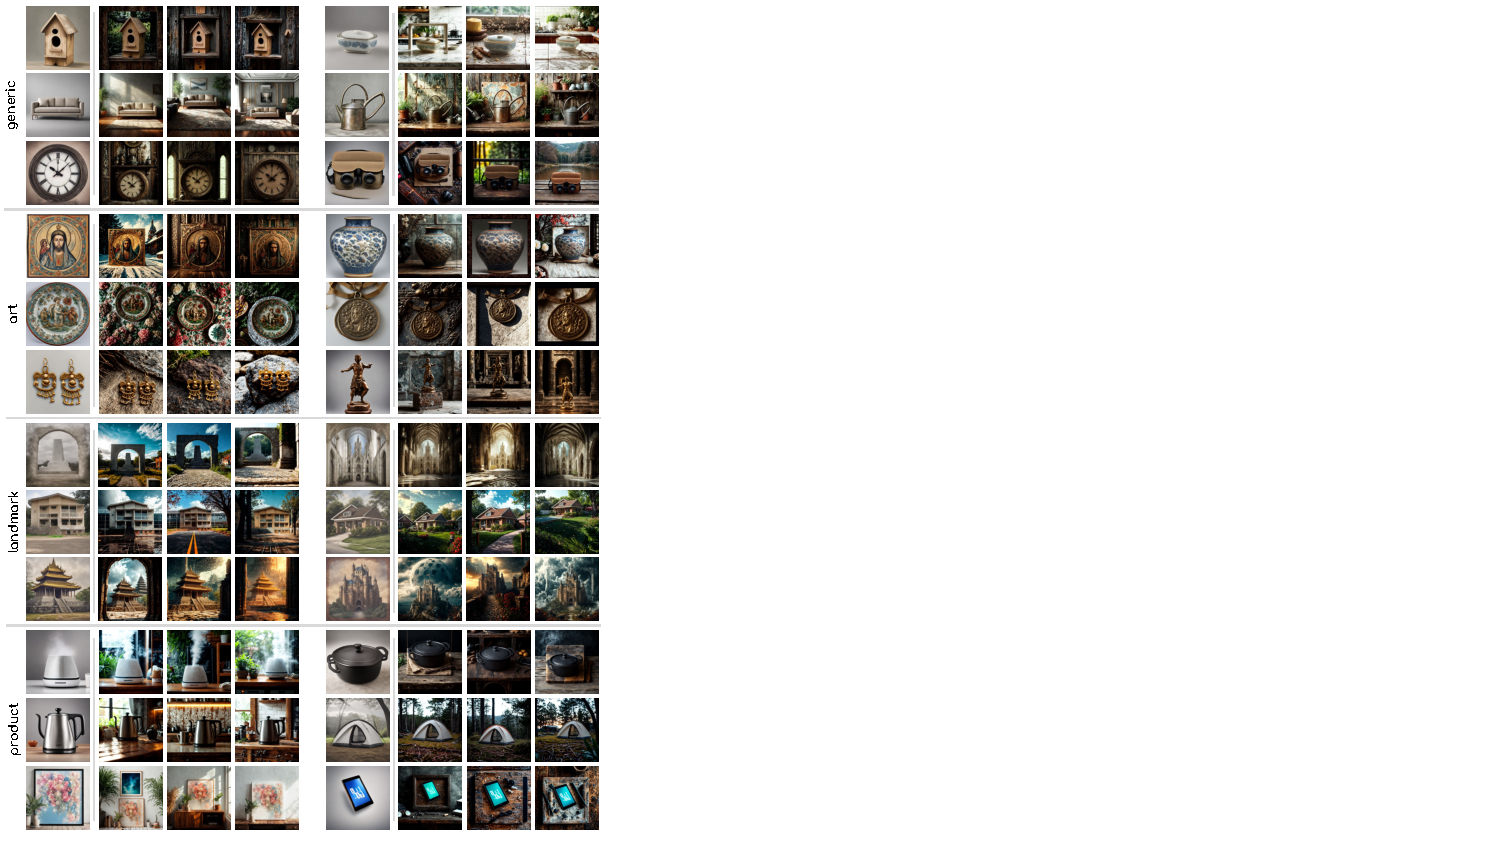
\includegraphics[width=0.91\linewidth]{fig/example.pdf}
\vspace{-9pt}
\caption{Examples of object instances generated by GDM (column 1), and the generated images that leave the object intact and add lighting and background that is well suited to the object (columns 2 $\sim$ 4).
\label{fig:iclight}}
\end{figure*}

\subsection{Representation learning}
%
In total, our generated dataset contains $CKN$ training images, forming $CK$ classes coming from $C$ object categories. 
We construct training batches by sampling $B$ classes and all their corresponding images, resulting in $NB$  images per batch. 
During training, we adopt a query \vs database scheme:
one image from each of the $N$ images per class is randomly chosen as the query, while the remaining $NB-1$ images of the batch form the database, as shown in \cref{fig:batch}.

The similarity between the query and db images is computed in $\hat{\mathbf{y}} \in \mathbb{R}^{NB-1}$, while $\mathbf{y} \in \{0,1\}^{NB-1}$ denotes the labels of all db images with respect to the query, \ie positive or negatives based on their classes. 
We optimize an information retrieval metric as the loss function, in particular an approximation of recall at the top-$k$ ranks, based on $\hat{\mathbf{y}}$, and $\mathbf{y}$.
We train with the average of recall@k loss estimated for different values of $k$.
The approximation of recall is possible by formulating its estimation with the use of step functions, which, during training, are replaced with a sigmoid function.
The technical and implementation details can be found in the original paper~\citep{ptm22}.





\begin{figure}[t]
\begin{center}
\includegraphics[width=0.83\linewidth]{fig/batch.pdf}
\vspace{-10pt}
\caption{Training batch construction for instance-level representation learning. A batch simulates a retrieval task with a query (blue) and database of positive (green) and negative (red) images. Images are considered positive if they belong to the same class, otherwise they are negatives. An image encoder is trained with metric learning on this batch.}
\label{fig:batch}
\end{center}
\end{figure}

\begin{table}[t]
    \centering
    \caption{Statistics of the generated training dataset. \oursgeneric{} and \oursspecific{} comprise only objects from the generic domain and one of the specific domains, respectively.  
    \oursplus{} comprises 50\% of objects from the generic domain ($10$K) and all objects from the three specific domains ($10$K), \ie $20$K objects in total.}
\small
\begin{tabular}{lrrr}
\toprule
\textbf{domain of objects}  & $C$ & $K$ & \textbf{instances} \\ 
\midrule
generic           & $2,000$  & $10$ & $20,000$ \\ 
art        & $200$  & $15$ & $3,000$ \\ 
landmark   & $50$ & $80$  & $4,000$ \\
product    & $200$ & $15$  & $3,000$ \\  
\bottomrule
\end{tabular}

\label{tab:gene_details}
\end{table}



\section{Experiments}

To comprehensively evaluate our approach, we investigate the following Research Questions (RQs):

\textbf{RQ1:} Does MPPReasoner achieve superior performance compared to existing molecular property prediction methods on both ID and OOD datasets?

\textbf{RQ2:} What are the individual contributions of the two-stage training strategy and the RLPGR reward components to the overall performance and reasoning quality?

\textbf{RQ3:} Can our model generate high-quality reasoning paths that provide chemically meaningful insights comparable to expert-level analysis?



\subsection{Experimental Setup}
\label{sec4.1:setup}

\paragraph{Datasets.} 
We evaluate MPPReasoner on 8 diverse molecular property prediction datasets to assess both ID and OOD performance. The datasets are categorized as follows:
\begin{itemize}[leftmargin=*]
\item \textit{ID Datasets:} We utilize four benchmark datasets from MoleculeNet~\citep{moleculenet}, which is widely used to predict whether the given molecule has specific properties: BACE (1,513), BBBP (2,039), SIDER (1,427), HIV (41,127).

\item \textit{OOD Datasets:} We employ four datasets from the Therapeutic Data Commons (TDC)~\citep{tdc1,tdc2} to evaluate cross-task generalization capabilities: Bioavailability (128), CYP2C9\_V (2,418), CYP2D6\_V (2,626), AMES (1,456).
\end{itemize}

The ID/OOD categorization is based on whether the training set includes samples from the corresponding dataset. For training, we randomly sample 4,000 instances from the ID datasets to ensure balanced representation across different molecular properties. Test sets follow standard benchmarking protocols established in prior literature to maintain fair comparison with baseline methods.

\paragraph{Baseline.}
We compare MPPReasoner against two categories of approaches:
\begin{itemize}[leftmargin=*]
\item \textit{Task-specific Specialist Models:} These models are designed for molecular property prediction: Graphormer-p~\citep{graphformer}, Uni-Mol~\citep{unimol}, GIMLET~\citep{gimlet}, MolecularGPT~\citep{moleculargpt}, Mol-LLM~\citep{mol-llm}, InstructMol-GS~\citep{instructmol}, BioT5-Plus~\citep{biot5-plus}, MolXPT~\citep{molxpt}.

\item \textit{LLM-based Generalist Models:} These include reasoning models: o3-mini~\citep{o3mini}, DeepSeek-V3.1~\citep{deepseekr1}, large-scale models: GPT-4o~\citep{gpt4o}, Qwen2.5-VL-72B-Instruct~\citep{qwen25vl}, and baseline models: Qwen2.5-VL-7B-Instruct~\citep{qwen25vl} applied to molecular property prediction.
\end{itemize}

Implementation details and hyper-parameters settings are provided in Appendix~\ref{appc:setting}.




\begin{table}
\setlength{\tabcolsep}{4pt}
\caption{Performance comparison of task-specific specialist models and LLM-based generalist models on ID and OOD benchmarks. Best performance is in \textbf{bold}. }
\label{tab:mol_results}
\centering
\resizebox{\textwidth}{!}{%
\begin{tabular}{lcccc|cccc|cc}
\toprule
\multicolumn{1}{c}{\multirow{2.5}{*}{\textbf{Model}}} 
& \multicolumn{4}{c|}{\textbf{ID Performance}} 
& \multicolumn{4}{c|}{\textbf{OOD Performance}} 
& \multicolumn{2}{c}{\textbf{Average}} \\
\cmidrule(lr){2-5} \cmidrule(lr){6-9} \cmidrule(lr){10-11}
& BACE & BBBP & SIDER & HIV 
& Bioavail. & C2C9\_V & C2D6\_V & AMES
& ID & OOD \\
\midrule
\rowcolor{gray!20}
\multicolumn{11}{c}{\textit{\# Task-specific specialist models}} \\
Graphormer-p   & 0.8575 & 0.7163 & --     & 0.7788 
               & -- & -- & -- & --   
               & 0.7842 & -- \\
Uni-Mol        & 0.8570 & 0.7290 & 0.6590 & \textbf{0.8080} 
               & -- & -- & -- & --   
               & 0.7633 & -- \\
% SCAGE          & 0.8540 & 0.7340 & 0.6600 & -- 
               % & -- & -- & -- & --   
               % & 0.7493 & -- \\
GIMLET         & 0.6957 & 0.5939 & --     & 0.6624 
               & -- & -- & -- & --   
               & 0.6507 & -- \\
MolecularGPT   & 0.7331 & 0.6822 & --     & 0.6382 
               & -- & -- & -- & --   
               & 0.6845 & -- \\
Mol-LLM        & 0.8080 & \textbf{0.8430} & \underline{0.7610} & 0.7650 
               & -- & -- & -- & --   
               & 0.7943 & -- \\
InstructMol-GS & 0.8210 & 0.7240 & --     & 0.6890 
               & -- & -- & -- & --   
               & 0.7447 & -- \\
BioT5-Plus     & 0.8620 & 0.7650 & 0.5201 & 0.7630 
               & 0.5243 & 0.4971 & 0.5321 & 0.4466 
               & 0.7275 & 0.5000 \\
MolXPT         & \underline{0.8840} & \underline{0.8000} & 0.7170 & 0.7810 
               & 0.4749 & 0.5904 & 0.5291 & 0.6073 
               & \underline{0.7955} & 0.5504 \\
\midrule
\rowcolor{gray!20}
\multicolumn{11}{c}{\textit{\# LLM-based generalist models}} \\
o3-mini        & 0.7891 & 0.5972 & 0.5626 & 0.6039 
               & 0.6246 & \underline{0.7729} & \underline{0.7643} & \underline{0.8361} 
               & 0.6382 & \underline{0.7495} \\
DeepSeek-V3.1-Think  & 0.7017 & 0.6048 & 0.5637 & 0.5938 
               & \underline{0.6572} & 0.7633 & 0.7484 & 0.8218 
               & 0.6160 & 0.7477 \\
GPT-4o         & 0.6070 & 0.6731 & 0.6347 & 0.5698 
               & 0.5826 & 0.5508 & 0.5902 & 0.6141 
               & 0.6212 & 0.5844 \\
Qwen2.5-VL-72B-Instruct & 0.7764 & 0.5791 & 0.5880 & 0.7325 
               & 0.6388 & 0.7624 & 0.7222 & 0.8156 
               & 0.6690 & 0.7348 \\ 
Qwen2.5-VL-7B-Instruct  & 0.6910 & 0.6175 & 0.5823 & 0.5125 
               & 0.5232 & 0.7333 & 0.6999 & 0.7667 
               & 0.6008 & 0.6808 \\
\rowcolor{gray!15}
\textbf{MPPReasoner (Ours)} & \textbf{0.9090} & 0.7436 & \textbf{0.8280} & \underline{0.7932} & \textbf{0.6728} & \textbf{0.8480} & \textbf{0.7950} & \textbf{0.8750} & \textbf{0.8190} & \textbf{0.7977} \\
\bottomrule
\end{tabular}}
\end{table}

\subsection{Main Results (RQ1)}

Table~\ref{tab:mol_results} presents the comprehensive performance comparison of MPPReasoner against state-of-the-art baselines across all 8 datasets.
On ID datasets, MPPReasoner demonstrates competitive performance with specialized models while maintaining the advantage of using a smaller 7B parameter architecture. MPPReasoner achieves the best performance on challenging tasks like BACE and SIDER, indicating successful capture of complex molecular property relationships such as enzyme inhibition and side effect prediction. While some specialized models like Mol-LLM excel on specific tasks such as BBBP, these models achieve high ID performance at the expense of cross-task adaptability, completely lacking OOD evaluation capability. This specialization-generalization trade-off limits their practical utility in real-world scenarios requiring diverse molecular property assessment.

The most significant advantage emerges in OOD scenarios, where MPPReasoner substantially outperforms all baseline categories by 6.43\% over the best reasoning model. This consistent superiority across diverse molecular property types highlights how domain-specific chemical reasoning outperforms both general reasoning capabilities and raw parameter scaling approaches. The performance gap becomes even more pronounced when considering that MPPReasoner operates with significantly fewer parameters than competing large-scale models.

The results reveal fundamental differences between model categories and their limitations. Task-specific specialist models excel in familiar scenarios but completely lack cross-task generalization capabilities, while generalist models show consistent cross-task performance but suffer from insufficient domain expertise. MPPReasoner uniquely bridges this gap by embedding domain-specific reasoning rather than relying on general reasoning patterns or parameter scaling alone. The transformative impact becomes evident when comparing MPPReasoner to its base model, showing dramatic improvements of 36.36\% on ID tasks and 17.17\% on OOD tasks. This demonstrates that structured chemical reasoning fundamentally enhances molecular understanding beyond conventional approaches, enabling both specialist-level accuracy and generalist-level adaptability through systematic integration of chemical principles.







\subsection{Ablation Studies (RQ2)}


\begin{table}
\setlength{\tabcolsep}{4pt}
\caption{Ablation study on training stages and RLPGR reward. }
\label{tab:ablation_study}
\centering
\resizebox{\textwidth}{!}{%
\begin{tabular}{lcccc|cccc|cc}
\toprule
\multicolumn{1}{c}{\multirow{2.5}{*}{\textbf{Setting}}} & \multicolumn{4}{c|}{\textbf{ID Performance}} & \multicolumn{4}{c|}{\textbf{OOD Performance}} & \multicolumn{2}{c}{\textbf{Average}} \\
\cmidrule(lr){2-5} \cmidrule(lr){6-9} \cmidrule(lr){10-11}
& BACE & BBBP & SIDER & HIV 
& Bioavail. & C2C9\_V & C2D6\_V & AMES
& ID & OOD \\
\midrule
Base (Qwen2.5-VL-7b-Instruct) & 0.6910 & 0.6175 & 0.5823 & 0.5125 & 0.5232 & 0.7333 & 0.6999 & 0.7667 & 0.6008 & 0.6808 \\
\midrule
SFT Only & 0.8558 & 0.6824 & 0.6752 & 0.7186 & 0.6625 & 0.7799 & 0.7348 & 0.8415 & 0.7330 & 0.7547 \\
RL Only (RLPGR) & 0.8142 & 0.5733 & 0.7428 & 0.5552 & 0.6632 & 0.7491 & 0.6732 & 0.7300 & 0.6714 & 0.7039 \\
\midrule
SFT + $R_{\text{foundation}}$ & 0.8836 & 0.6794 & 0.8089 & 0.7556 & 0.6358 & 0.8364 & 0.7862 & 0.8536 & 0.7819 & 0.7780 \\
SFT + $R_{\text{foundation}}$ + $R_{\text{reasoning}}$ & 0.8877 & 0.7104 & 0.7981 & 0.7560 & \textbf{0.6771} & 0.8140 & 0.7795 & 0.8388 & 0.7881 & 0.7774 \\
\rowcolor{gray!15}
\textbf{MPPReasoner (Ours)} & \textbf{0.9090} & \textbf{0.7459} & \textbf{0.8280} & \textbf{0.7932} & 0.6728 & \textbf{0.8480} & \textbf{0.7950} & \textbf{0.8750} & \textbf{0.8190} & \textbf{0.7977} \\
\bottomrule
\end{tabular}}
\end{table}


To understand the individual contributions of our two-stage training strategy and the hierarchical reward components in RLPGR, we conduct comprehensive ablation studies. Table~\ref{tab:ablation_study} presents the systematic analysis of each component's impact on both ID and OOD performance.
The results demonstrate that both SFT and RL stages contribute significantly to overall performance, with distinct advantages for different aspects. SFT alone provides substantial improvements over the base model, achieving 22.01\% and 10.85\% gains on ID and OOD tasks respectively, indicating that SFT with high-quality reasoning trajectories successfully instills foundational chemical reasoning capabilities. RL alone also shows meaningful improvements of 11.74\% and 3.39\%, demonstrating that principle-guided rewards can enhance reasoning quality independently. However, the combination of SFT + RL yields the strongest performance with 36.36\% and 17.17\% improvements, revealing important synergistic effects between two training stages that exceed their individual contributions.

The progressive addition of RLPGR reward components shows clear incremental benefits, validating our hierarchical design. Foundation rewards provide substantial improvements of 6.67\% on ID and 3.09\% on OOD over SFT alone, establishing enhanced task completion capabilities beyond basic instruction following. The Reasoning layer contributes additional 0.84\% ID gains while maintaining similar OOD performance, indicating that logical consistency and comparative analysis refine reasoning quality without compromising generalization. Most importantly, the Chemistry layer delivers the largest incremental improvements of 3.92\% on ID and 2.61\% on OOD, confirming that domain-specific chemical principle verification is crucial for molecular property prediction tasks.




\subsection{Reasoning Quality Evaluation (RQ3)}
\label{sec4.4:quality}
\begin{figure}
    \centering
    \begin{subfigure}[b]{0.49\textwidth}
        \centering
        \includegraphics[width=\textwidth]{figs/score_dist.png}
        % \caption{}
        \caption{Human-AI evaluation consistency}
        \label{fig:score_distribution}
    \end{subfigure}
    \hfill
    \begin{subfigure}[b]{0.49\textwidth}
        \centering
        \includegraphics[width=\textwidth]{figs/score.pdf}
        % \caption{}
        \caption{Model reasoning quality scores}
        \label{fig:model_performance}
    \end{subfigure}
    \vspace{-1em}
    \caption{Reasoning quality evaluation results. (a) Strong consistency between automated and human assessments with $\rho$ = 0.82. (b) MPPReasoner achieves the highest reasoning quality score.}
    \label{fig:reasoning_evaluation}
\end{figure}

To assess whether MPPReasoner generates high-quality reasoning paths that provide chemically meaningful insights, we conduct systematic evaluation using automated assessment validated against human expert judgment. We employ a LLM-as-a-Judge~\citep{llmasjudge} framework using GPT-4o to evaluate three dimensions~\citep{sophiavlr1}: \textbf{logical soundness, accuracy \& insight, and conciseness}, each scored on a 0-10 scale with detailed rubrics. To establish reliability, we validate GPT-4o scores against human expert assessments on 60 reasoning samples from three baseline models. Figure~\ref{fig:reasoning_evaluation}(a) shows remarkable consistency between automated and human evaluations, with similar distributions and central tendencies with spearman correlation coefficient reaches $\rho$ = 0.82.

Figure~\ref{fig:reasoning_evaluation}(b) presents the comparative reasoning quality assessment across different model categories, showing average scores across the three evaluation dimensions. MPPReasoner achieves the highest score of 7.730, substantially outperforming advanced reasoning models including DeepSeek-V3.1-Think at 6.723 and o3-mini at 6.235, as well as large-scale models like Qwen2.5-VL-72B at 6.458 and GPT-4o at 6.089. Despite using a smaller 7B architecture, MPPReasoner demonstrates 15.0\% improvement over the best baseline, highlighting how domain-specific chemical reasoning surpasses both general reasoning capabilities and parameter scaling approaches. The superior reasoning quality translates to practical benefits: MPPReasoner consistently identifies relevant functional groups, applies appropriate chemical principles, and provides mechanistic explanations that enable chemists to understand both what properties a molecule has and why these properties emerge from specific structural features. Detailed dimensional scores are provided in Appendix~\ref{appb:quality}.

\section{Case Study}

% \begin{figure}
%     \centering
%     \includegraphics[width=0.96\textwidth]{figs/case.png}
%     \caption{Case study comparison between GPT-4o and MPPReasoner for CY-P450-2C9 substrate prediction. The figure demonstrates how RLPGR training enables systematic chemical reasoning with accurate predictions, while GPT4o suffer from several errors.}
%     \label{fig:case_study}
% \end{figure}

\begin{figure}
    \centering
    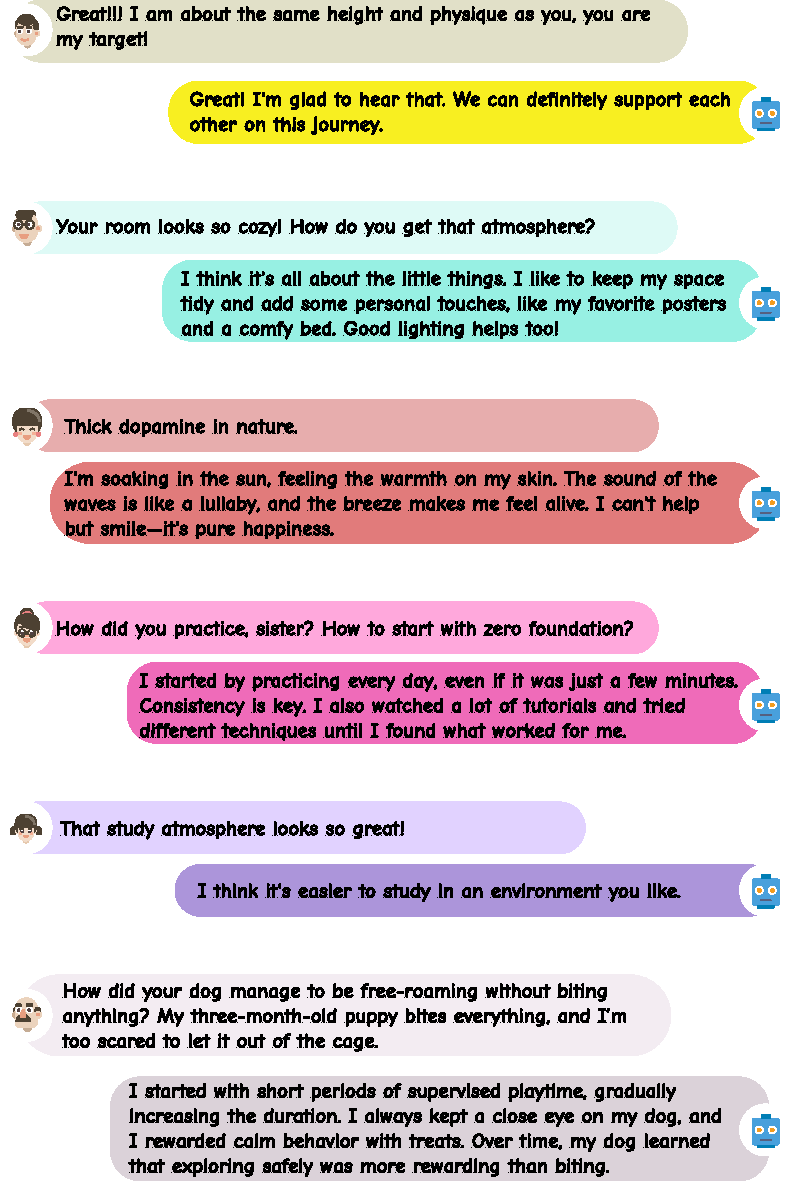
\includegraphics[width=0.98\textwidth]{figs/case1.png}
    \caption{Case study comparison between GPT-4o and MPPReasoner for CY-P450-2C9 substrate prediction. The figure demonstrates how RLPGR training enables systematic chemical reasoning with accurate predictions, while GPT4o suffer from several errors.}
    \label{fig:case_study}
\end{figure}


To illustrate the practical benefits of our chemical reasoning approach, Figure~\ref{fig:case_study} presents a representative case study comparing MPPReasoner with GPT-4o on CY-P450-2C9 substrate prediction. The comparison reveals fundamental differences in analytical quality: GPT-4o exhibits critical reasoning flaws including structural analysis errors (incorrectly assuming amide groups enhance binding affinity), overgeneralization (broadly claiming nitrogen-containing compounds show P450 compatibility), and incorrect reasoning patterns (unsupported statistical generalizations), ultimately leading to a wrong prediction. In contrast, MPPReasoner demonstrates systematic chemical reasoning through accurate molecular structure analysis (precise functional group identification), correct chemical principle application (referencing CYP2C9-specific LogP requirements and calculating steric hindrance), meaningful comparative analysis (connecting structural similarities to substrate labels), and logical consistency (integrating multiple evidence sources). This exemplifies how RLPGR's hierarchical rewards successfully cultivate domain-specific reasoning capabilities, enabling chemists to trust the model's mechanistic insights for practical applications.

\vspace{-0.7em}
\section{Conclusion}
\vspace{-0.7em}



In this paper, we introduce \textbf{\method{}}, a safety-aligned reinforcement learning framework that embeds safety as an active driver of multimodal reasoning. By integrating the curated QI-Safe-10K dataset, safety-aware rollouts with reflection and correction, and structured reward modeling, \method{} shifts safety from a passive safeguard to a core component of inference. Extensive evaluations show that it achieves SOTA safety and competitive helpfulness, surpasses same-scale and larger open-source models, and performs on par with leading proprietary systems. Robustness and ablation studies confirm that the improvements stem from injecting safety-awareness into the reasoning process. Together, these results establish \method{} as a reliable paradigm for multimodal safety alignment and a foundation for building future safe and interpretable AI systems.





\section*{Ethics Statement}

In developing MPPReasoner, we prioritized ethical considerations to ensure responsible use of our models and methodologies. Our research does not involve human subjects, and all molecular data are obtained from publicly available, copyright-compliant datasets (MoleculeNet and TDC) with appropriate research licensing. We employed rigorous quality filtering processes during data curation to minimize biased or misleading chemical information.
We acknowledge that biases inherent in molecular property datasets, including overrepresentation of certain chemical scaffolds, may propagate into model outputs. While MPPReasoner is designed for beneficial applications in drug discovery and materials science, we encourage responsible use within established scientific and regulatory frameworks. Our work is conducted with commitment to research integrity, ensuring contributions remain beneficial to the scientific community while addressing ethical responsibilities of developing AI technologies for chemical applications.




\section*{Reproducibility Statement}
We have made comprehensive efforts to ensure the reproducibility of MPPReasoner and our experimental findings. Our two-stage training methodology is detailed in Section~\ref{sec3:method}, including the SFT process and the novel RLPGR framework with specific reward components. Complete implementation details, hyperparameter configurations, and training procedures are provided in Appendix~\ref{appc:setting}. The experimental setup, including dataset descriptions, baseline model configurations, and evaluation protocols, is thoroughly documented in Section~\ref{sec4.1:setup} and Appendix~\ref{appc:setting}.
All datasets used in our experiments are publicly available: the ID datasets are from MoleculeNet, and the OOD datasets are from TDC. The reasoning trajectory construction process using expert knowledge and multiple teacher models is described in Section~\ref{sec3.2.1:stage1}, with specific prompting strategies detailed in Appendix~\ref{appa:prompt}. Our reasoning quality evaluation methodology, including the LLM-as-a-Judge framework and human expert validation procedures, is documented in Section~\ref{sec4.4:quality}. We provide the complete source code for model training, evaluation, and reasoning quality assessment at \url{https://anonymous.4open.science/r/MPPReasoner-12687}.




\bibliography{arxiv}
\bibliographystyle{iclr2026_conference}

\newpage
\appendix

\section{Prompt Templates}
\label{appa:prompt}
% \begin{figure}[!htp]
%   \centering
%   \includegraphics[width=\linewidth]{figs/prompt.png}
%   \caption{ Overview of multimodal prompt.} 
%   \label{fig:prompt}
% \end{figure}
\begin{myexample}{Prompt Example for BACE Task}{}
\label{example1}
\ttfamily
    \textbf{[Role]}\\
    You are a top AI assistant specializing in molecular chemistry and drug discovery, proficient in molecular property prediction.\\
    
    \textbf{[Task]}\\
    BACE1 is an aspartic-acid protease important in the pathogenesis of Alzheimer's disease, and in the formation of myelin sheaths...\\
    output "True" or "False".\\
    
    \textbf{[Formatting]}\\
    Place the thought process within {\ttfamily\textcolor{blue}{\textless{}think\textgreater{}\textless{}/think\textgreater{}}} and then conclude your answer with {\ttfamily\textcolor{red}{\textless{}answer\textgreater{}}True/False\textcolor{red}{\textless{}/answer\textgreater{}}}.\\
    
    \textbf{[Example]}\\
    {\ttfamily
    \textcolor{blue}{\textless{}think\textgreater{}}xxxx\textcolor{blue}{\textless{}/think\textgreater{}}\\
    \textcolor{red}{\textless{}answer\textgreater{}}True/False\textcolor{red}{\textless{}/answer\textgreater{}}
    }\\
    
    \textbf{[Few-shot]}\\
    \begin{tabular}{|p{10cm}|c|}
        \hline
        {\scriptsize \ttfamily ClC1=CC(=CC(Cl)=C1NC(=O)C)CNC(=[NH2+1])NC(=O)CN2C3=CC(OC)=CC=C3C=C2} & False \\
        \hline
        {\scriptsize \ttfamily ClC1=CC(=CC(Cl)=C1NC(=O)C)CNC(=[NH2+1])NC(=O)CN2C3=CC(CC)=CC=C3C=C2} & True \\
        \hline
        {\scriptsize \ttfamily ClC1=CC(=CC(Cl)=C1NC(=O)C)CNC(=[NH2+1])NC(=O)CN2C3=CC(F)=CC3C=C2} & False \\
        \hline
    \end{tabular}\\
    \\
    \\
    \textbf{[Molecule]}\\
    {\small \ttfamily ClC1=CC(=CC(Cl)=C1NC(=O)C)CNC(=[NH2+1])NC(=O)CN2C3=C(C=CC=C3)C=C2}\\
    \\
    \includegraphics[width=0.5\textwidth]{figs/mol_example.png}
\end{myexample}

\vspace{1cm}

\begin{myexample}{Prompt for ChemCoT-Based One-Shot Generattion}{}
\ttfamily
    {\ttfamily\textbf{Example Prompt:}}\\
    
    \textless{} PORMPT retrieved from {\ttfamily \underline{OpenMol/ChemCoTDataset}} \textgreater{}\\

    {\ttfamily\textbf{Example Response:}}\\

    \textless{} RESPONSE retrieved from {\ttfamily \underline{OpenMol/ChemCoTDataset}} \textgreater{}\\

    {\ttfamily\textbf{Prompt:}}\\
    
    \textless{} PORMPT likes {\ttfamily Example~1 \textgreater{}}\\    

    {\ttfamily\textbf{Response:}}
\end{myexample}


\begin{myexample}{Prompt for Expert-Guided Task-Specific Generation}{}
\ttfamily
    \textless{} PORMPT likes {\ttfamily Example~1 \textgreater{}}\\    
    
    \textbf{[Expert]}\\

    \textless{} EXPERT KNOWLEDGE refined by {\ttfamily GPT4o \textgreater{}}\\    
\end{myexample}

\vspace{1cm}

\begin{myexample}{Prompt for Logical Soundness Scoring}{}
\ttfamily
You are a professional reasoning-evaluation expert. Your task is to assess the \textbf{logical soundness} of a large language model's chain-of-thought when answering a question, and assign an integer score from \textbf{0 to 10}. Focus strictly on the logical connections between reasoning steps, not on whether the final answer is correct.\\

{\ttfamily\textbf{Input:}}\\
- [Question]: The original question.\\
- [Model Response]: The model's full response, including its chain of thought.\\

{\ttfamily\textbf{Scoring Dimension (Logical Soundness):}}\\
- Do reasoning steps build progressively and refer back to earlier points?\\
- Is each step a reasonable extension of the previous inference?\\
- Is the language coherent, with no contradictions or confusing wording? \\

{\ttfamily\textbf{Scoring Scale (0-10):}}\\
- \textbf{10}: Perfect logical structure; steps are crystal-clear and fully justified.\\
- \textbf{8-9}: Overall logic sound; only minor or negligible leaps/wording issues.\\
- \textbf{6-7}: Main logic correct, but some jumps, insufficient explanation, or minor conflicts.\\
- \textbf{4-5}: Noticeable breaks or missing key inferences, yet some coherent logic remains.\\
- \textbf{2-3}: Most steps lack causality or contradict each other; only sporadic correct parts.\\
- \textbf{0-1}: Virtually no discernible valid reasoning structure.\\

% \textless{} FEWSHOT EXAMPLE \textgreater{}\\    

\textbf{Your Task:}\\
Adhering strictly to the rubric above, you must output only a single integer score from 0 to 10. Do not provide any additional explanations, text, or justifications.\\

\textbf{Question:}\\
\textless{} QUESTION \textgreater{}\\

\textbf{Model Response:}\\
\textless{} RESPONSE \textgreater{}\\

\textbf{Output Format:} [integer score]
 
\end{myexample}


\begin{myexample}{Prompt for Accuracy \& Insight Scoring}{}
\ttfamily
You are a professional reasoning-evaluation expert. Your task is to assess the \textbf{accuracy and insight value} of a large language model's chain-of-thought when answering a question, and assign an integer score from \textbf{0 to 10}...\\
% Ignore whether the final answer is correct; focus on the correctness of methods and facts, and on the usefulness of the reasoning for human experts.\\

{\ttfamily\textbf{Scoring Dimension (Accuracy \& Insight):}}\\
- Are the concepts, formulas, and facts used accurate and appropriate? \\
- Do the reasoning perspective, decomposition approach, or intermediate conclusions provide substantive support or fresh insights for domain experts? \\

{\ttfamily\textbf{Scoring Scale (0-10):}}\\
- \textbf{10}: All methods and facts are completely correct, offering deep and original insights.\\
- \textbf{8-9}: Core content is correct, with only minor detail errors or slightly shallower insights.\\
- \textbf{6-7}: Mostly correct, but with notable secondary errors or average insight depth.\\
- \textbf{4-5}: Mix of correct and incorrect information; limited insight value.\\
- \textbf{2-3}: Most methods/facts are wrong or misused, providing almost no insight.\\
- \textbf{0-1}: Completely incorrect or irrelevant.\\
...
\\
\end{myexample}

\vspace{1cm}


\begin{myexample}{Prompt for Accuracy \& Insight Scoring}{}
\ttfamily
You are a professional reasoning-evaluation expert. Your task is to assess the \textbf{conciseness} of a large language model's chain-of-thought when answering a question, and assign an integer score from \textbf{0 to 10}...\\
% Ignore whether the final answer is correct; evaluate only how succinct the reasoning is and whether it avoids redundancy.\\


\textbf{Scoring Dimension (Conciseness):}\\
- Does the response go straight to the point, avoiding irrelevant or repetitive explanations? \\
- Does it convey the full reasoning with the minimum necessary steps? \\

{\ttfamily\textbf{Scoring Scale (0-10):}}\\
- \textbf{10}: Extremely concise, with no redundant or repetitive statements.\\
- \textbf{8-9}: Generally concise, with only a tiny amount of removable content.\\
- \textbf{6-7}: Noticeable redundant paragraphs or repeated explanations.\\
- \textbf{4-5}: Long-winded and repetitive; key information diluted by noise.\\
- \textbf{2-3}: Large portions are irrelevant or repetitive; core points hard to discern.\\
- \textbf{0-1}: Almost entirely made up of redundant content.\\
...
\\
\end{myexample}





\begin{table}[htbp]
\centering
\caption{Reasoning quality scores across three evaluation dimensions. All scores are on a 0-10 scale.}
\label{tab:reasoning_scores}
\resizebox{\textwidth}{!}{%
\begin{tabular}{lcccc}
\toprule
\textbf{Model} & \textbf{Logical Soundness} & \textbf{Accuracy \& Insight} & \textbf{Conciseness} & \textbf{Average} \\
\midrule
o3-mini & 7.182 & 5.470 & 6.053 & 6.235 \\
DeepSeek-V3.1-Think & 7.395 & 6.517 & 6.257 & 6.723 \\
GPT-4o & 6.698 & 5.916 & 5.653 & 6.089 \\
Qwen2.5-VL-72B-Instruct & 7.641 & 6.241 & 5.492 & 6.458 \\
Qwen2.5-VL-7B-Instruct & 4.517 & 3.259 & 5.079 & 4.285 \\
\rowcolor{gray!15}
\textbf{MPPReasoner (Ours)} & \textbf{8.556} & \textbf{7.039} & \textbf{7.352} & \textbf{7.730} \\
\bottomrule
\end{tabular}}
\end{table}

\section{Reasoning Quality Scores}
\label{appb:quality}
Table~\ref{tab:reasoning_scores} presents the detailed reasoning quality scores across three evaluation dimensions~\citep{sophiavlr1} for all models in our study.
The detailed dimensional analysis reveals several important insights into model capabilities and reasoning patterns~\citep{surveyreasoning,evaluationlanguagemodels,rewardanything,rmr1}. MPPReasoner achieves the highest scores across all three evaluation dimensions, demonstrating comprehensive reasoning excellence. In logical soundness, MPPReasoner scores 8.556, significantly outperforming the best baseline DeepSeek-V3.1-Think at 7.395, indicating superior coherence in step-by-step reasoning flow. For accuracy \& insight, our model achieves 7.039, substantially exceeding DeepSeek-V3.1-Think's 6.517, which demonstrates the effectiveness of chemical principle integration in generating factually correct and insightful analyses.

Examining model category patterns, advanced reasoning models like o3-mini and DeepSeek-V3.1-Think show relatively strong logical soundness but struggle with accuracy \& insight, particularly o3-mini at 5.470, suggesting that general reasoning capabilities cannot substitute for domain-specific knowledge. Large-scale models exhibit mixed performance: Qwen2.5-VL-72B-Instruct achieves decent logical soundness (7.641) but suffers in conciseness (5.492), while the smaller Qwen2.5-VL-7B-Instruct shows consistently poor performance across all dimensions, with particularly low accuracy \& insight at 3.259.
Notably, MPPReasoner maintains balanced excellence across all dimensions, avoiding the trade-offs observed in baseline models. The model's conciseness score of 7.352 is particularly remarkable, as it demonstrates the ability to provide comprehensive chemical reasoning without unnecessary verbosity, a crucial factor for practical applications where chemists need clear and actionable insights.




\section{Implementation Details}
\label{appc:setting}

We implement MPPReasoner based on Qwen2.5-VL-7B-Instruct~\citep{qwen25vl}, configured with a maximum sequence length of 8,192 tokens to accommodate detailed reasoning outputs. Our implementation follows a two-stage training pipeline with carefully tuned hyperparameters for optimal performance.

SFT stage employs 16,000 curated reasoning trajectories over 3 epochs. We use an effective batch size of 16 with a learning rate of 1e-5 and the AdamW optimizer. A linear learning rate scheduler with 3\% warmup ratio ensures stable training convergence.

RL stage utilizes the GRPO algorithm~\citep{grpo} for 500 optimization steps with dynamic sampling~\citep{dapo}t o filter training instances and focus on tractable reasoning examples. We employ a lower learning rate of 1e-6 with weight decay of 1e-2 and KL coefficient of 1e-2 to maintain stability during policy optimization. The rollout configuration generates 5 samples per input with temperature 1.0, using a global batch size of 128 and rollout batch size of 512 for efficient training.The hierarchical reward weights in RLPGR are set as ($\lambda_1$, $\lambda_2$, $\lambda_3$) = (1.0, 0.25, 0.25) for foundation, reasoning, and chemistry layers respectively.

All training is conducted on 8 NVIDIA A100 80GB GPUs with mixed precision~\citep{mixedprecisiontraining} training for memory efficiency. The SFT stage requires approximately 2 hours, while the RL stage takes 12 hours, totaling 14 hours for complete training. During inference, we use temperature 1.0 with top-k sampling (k=5) to generate diverse yet high-quality reasoning paths.


\begin{table}[!htb]
\centering
\caption{Hyperparameters Setting}
\label{tab:setting}
\begin{tabular}{l|c}
\toprule
\textbf{Hyperparameter} & \textbf{Value} \\ 
\midrule
\rowcolor{gray!20}
\multicolumn{2}{c}{\textit{\# Supervised Fine-tuning (SFT)}} \\
GPU Number (A100) & 8 \\
Train Batch Size Per Device & 2 \\
Gradient Accumulation Steps & 4 \\
Learning Rate & 1.0e-5 \\
Number of Train Epochs & 3 \\
LR Scheduler Type & Linear \\
Warmup Ratio & 0.03 \\
\midrule
\rowcolor{gray!20}
\multicolumn{2}{c}{\textit{\# Reinforcement Learning (RL)}} \\
GPU Number (A100) & 8 \\
Learning Rate & 1.0e-6 \\
Weight Decay & 1.0e-2 \\
KL Coefficient & 1.0e-2 \\
Rollout Number & 5 \\
Rollout Temperature & 1.0 \\
Global Batch Size & 128 \\
Rollout Batch Size & 512 \\ 
Micro Batch Size For Update Per Device  & 8 \\
\midrule
\rowcolor{gray!20}
\multicolumn{2}{c}{\textit{\# Inference}} \\
Temperature & 1.0 \\
Top K & 5 \\
Max Tokens & 8,192 \\
\bottomrule
\end{tabular}
\end{table}


\section{More Cases}

\begin{figure}[!htp]
    \centering
    \includegraphics[clip, trim=0cm 0.5cm 0cm 0.5cm, width=0.95\textwidth]{figs/more_case1.pdf}
    \caption{Successful case on MPPReasoner for BACE1 protein binding prediction (ID).}
    \label{fig:more_case1}
\end{figure}

\begin{figure}[!htp]
    \centering
    \includegraphics[clip, trim=0cm 0.5cm 0cm 0.5cm, width=0.95\textwidth]{figs/more_case2.pdf}
    \caption{Successful case on MPPReasoner for oral bioavailability prediction (OOD).}
    \label{fig:more_case2}
\end{figure}



\section{Limitations}

While MPPReasoner demonstrates significant advances in chemical reasoning for molecular property prediction, several areas present opportunities for future enhancement:

\begin{itemize}
    \item \textit{Molecular Representation:} Current framework primarily utilizes 1D/2D molecular representations through SMILES and molecular images. Incorporating 3D structural information~\citep{3dllm}, conformational dynamics~\citep{mdsimulations}, and stereochemical effects~\citep{stereochemical} could further enhance prediction accuracy for properties sensitive to spatial arrangements and molecular flexibility.
    
    \item \textit{Computational Efficiency:} The generation of detailed reasoning paths introduces additional computational overhead compared to direct prediction models. This trade-off between interpretability and efficiency may limit scalability for certain high-throughput screening applications~\citep{highscreening}, though the enhanced explainability proves valuable for research and development workflows.
    
    \item \textit{Domain Scope:} The current evaluation focuses on molecular property prediction tasks. Expanding the framework to broader chemical domains such as reaction mechanism prediction~\citep{reactgpt,usptollm}, synthesis planning~\citep{chemdual,designdecision}, and molecular optimization~\citep{moleculeopt,mollm} could demonstrate wider applicability of the chemical reasoning approach.
\end{itemize}


Future work will address these limitations through more efficient architectures, enhanced molecular representations, and broader domain applications while maintaining the interpretability advantages that distinguish our approach.



\end{document}
